\chapter{Abordagem meta-heurística para o TSP}

As seções a seguir descrevem algumas técnicas necessárias para implementar a meta-heuristica GILS-RVND --- descrita em \cite{SILVA2012513} --- visando solucionar instâncias do TSP. Embora tenha sido  proposta como uma solução para o \textit{Minimum Latency Problem} (MLP), essa meta-heurística também é capaz de obter boas soluções para o TSP quando implementada com as devidas adaptações.

\section{Preliminares}
Algumas observações devem devem ser feitas quanto à implementação do algoritmo.

\subsection{\textit{Standard Template Library}}
Ainda que o uso de programação orientada a objetos não seja obrigatório, a implementação da meta-heurística deve ser feita em C++. Para facilitar a implementação das estruturas de dados e rotinas necessárias no algoritmo, recomenda-se o estudo de alguns componentes da \textit{Standard Template Library} (STL), como \texttt{vector}, \texttt{list} e \texttt{sort()}.


\subsection{Diferença com o algoritmo descrito no artigo}
Mesmo que o MLP divirja do TSP em termos de complexidade e natureza, a maioria do algoritmo descrito em \cite{SILVA2012513} (em forma de pseudocódigo) pode ser aproveitada. Precisamente, os procedimentos devem ser implementados \textit{exatamente} como no algoritmo do artigo, exceto o procedimento de construção (\texttt{Construction(\(\alpha\))}), que deve ser implementado como descrito nas próximas seções.

\subsection{Leitor de instâncias}
Alguns arquivos de instâncias e o código de um leitor de instâncias --- que deve ser usado para facilitar a implementação do algoritmo ---  que calcula a matriz de distâncias se encontram neste link: \url{https://github.com/carlosvinicius01/kit-opt/tree/master/GILS-RVND-TSP}.

\subsection{Valores ótimos}
O valor ótimo de custo das instâncias fornecidas já foi determinado por meio de métodos exatos. Uma lista com esses valores --- que devem ser consultados para determinar a eficácia da implementação do algoritmo --- se encontra neste link: \url{http://elib.zib.de/pub/mp-testdata/tsp/tsplib/stsp-sol.html}.

Depois de implementado, o algoritmo deve ser capaz de obter o valor ótimo para instâncias de até 300 cidades na maioria das vezes em que é executado\footnote{Além de não garantir a obtenção de uma solução ótima, o algoritmo não é determinístico. Por isso, determinar a robustez e velocidade de sua implementação exige testá-lo extensivamente.}.

\subsection{Conceitos importantes}
Para compreender o algoritmo, é necessário, principalmente, saber o que são \textit{vizinhos}, \textit{movimentos} e \textit{estruturas de vizinhança}. Para isso, é recomendada a leitura dos capítulos 1 a 4 de \cite{MARCONE2011}.

\section{Representação de soluções}
Uma solução viável qualquer para o TSP pode ser pensada como uma sequência de cidades, cada uma visitada uma única vez. Considere \(V\) um conjunto de nós qualquer. Representando-se cada cidade como um nó \(i \in V\), sendo \(c_{ij}\) a distância entre as cidades \(i\) e \(j\) que por sua vez é associada a uma aresta \(e \in E\) , pode-se pensar no conjunto de soluções como um grafo \((V, E)\), e nas soluções viáveis como um ciclo Hamiltoniano.  

Considerando-se uma instância do TSP com 6 cidades, uma \linebreak solução viável \(s\) pode ser representada graficamente conforme a Figura \ref{fig:1}. A mesma solução \(s\) pode ser representada por meio da estrutura de dados na Figura \ref{fig:2}.



\begin{figure}[!htbp]
    \centering
    \begin{tikzpicture}
    
    \node[circle, draw=black] (v2) at (2,0) {2};
    \node[circle, draw=black] (v3) at (4,0) {3};
    \node[circle, draw=black] (v5) at (4,-4) {5};
    \node[circle, draw=black] (v6) at (2,-4) {6};
    
    
    \node[circle, draw=black] (v4) at (6,-2) {4};
    \node[circle, draw=black] (v1) at (0,-2) {1};
    
    \draw[-] (v1)--(v2);
    \draw[-] (v2)--(v3);
    \draw[-] (v3)--(v4);
    \draw[-] (v4)--(v5);
    \draw[-] (v5)--(v6);
    \draw[-] (v6)--(v1);
    
    \end{tikzpicture} 
    \caption{Solução viável de instância do TSP representada através de grafo.}
    \label{fig:1}
\end{figure}

\begin{figure}[H]
    \centering
    
        \begin{lstlisting}
std::vector<int> s = {1,2,3,4,5,6,1};
        \end{lstlisting}

    \caption{Solução viável de instância do TSP representada por meio de \texttt{vector}.}
    \label{fig:2}
\end{figure}

\section{Algoritmo principal}
O pseudocódigo do Algoritmo \ref{GILS-RVND-ALG} descreve a rotina principal da meta-heurística GILS-RVND.
\begin{algorithm}
\caption{GILS-RVND}\label{euclid}
\begin{algorithmic}[1]
\Procedure{GILS-RVND}{$I_{\text{Max}},I_{\text{ILS}}$}

\For{$i \gets 1,...,I_{\text{Max}}$}

\State \(\alpha \gets \text{valor aleatório } x \in [0, 1]\) 
\State \(s \gets \text{Construção}(\alpha)\)
\State \(s' \gets s\)
\State \(\text{\textit{IterILS}} \gets 0\)

\While{\(\text{\textit{IterILS}} < I_{\text{ILS}}\)}
\State \(s \gets \text{RVND}(s)\)

\If{\(f(s) < f(s')\)}
\State \(s' \gets s\)
\State \(\text{\textit{IterILS}} \gets 0\)
\EndIf

\State \(s \gets \text{Perturb}(s')\)
\State \(\text{\textit{IterILS}} \gets \text{\textit{IterILS}} + 1\)

\EndWhile

\If{\(f(s') < f(s^*)\)}
\State \(s^* \gets s'\)
\State \(f^* \gets f(s')\)
\EndIf

\EndFor

\EndProcedure
\end{algorithmic}
\label{GILS-RVND-ALG}
\end{algorithm}
    
\section{Construção}

\begin{algorithm}
\caption{Construção}\label{euclid}
\begin{algorithmic}[1]
\Procedure{Construção}{$\alpha$}
\State $ s \cup \{1\} $
\State \textit{CL} $\gets V \setminus \{1\}$  \Comment{Inicializa a lista de candidatos}

\For{$j \gets 1,...,3$} \Comment{Insere 3 cidades na solução aleatoriamente}
\State $i \gets$ nó aleatório de $CL$
\State $s \cup \{i\}$ \Comment{Concatena $s$ com $i$}
\State $CL \gets CL \setminus \{i\}$
\EndFor

\While{$CL \neq \emptyset$}
\State Inicializa a lista SD vazia; 
\For{$k \in CL$}
    \For{$(i, j) \gets (s_0, s_1), ..., (s_{|V|-1}, s_{|V|})$}
        \State custoInserção $\gets c_{ik} + c_{jk} - c_{ij}$
        \State SD $\gets \text{SD} \cup \{(\text{custoInserção}, k, (i, j))\}$
    \EndFor
\EndFor

\State Ordenar SD pelos custos de inserção
\State $s \gets \lfloor\alpha |\text{SD}|\rfloor$
\State $(c, v, (i,j)) \gets $ um dos primeiros $n$ elementos de SD, escolhido aleatoriamente
\State Insere a cidade $v$ na aresta $(i,j)$ de $s$
\State $CL \gets CL \setminus \{v\}$
\EndWhile

\State return $s$
\EndProcedure
\end{algorithmic}
\label{CONSTRUCAOD-ALG}
\end{algorithm}
    

O procedimento de obtenção de solução inicial --- ou construção --- que será utilizado se baseia no método GRASP, apresentado em \cite{MARCONE2011}. Nele, constrói-se uma solução inicial para o TSP começando-se com um \textit{subtour}\footnote{Um ciclo que não visita todas as cidades.}. Para isso, pode-se iniciar \(s\) com \texttt{\{1,1\}}, inserindo-se alguns nós \footnote{É suficiente iniciar a solução \(s\) com 3 nós aleatórios.} aleatoriamente em \(s\). O mesmo é demonstrado na Figura \ref{fig:3}, considerando novamente o exemplo com 6 cidades.

\begin{figure}
    \centering
    
    \begin{lstlisting}
std::vector<int> s = {1, 1};
std::vector<int> listaDeCandidatos = {2,3,4,5,6};
int tamanhoSubtourInicial = 3;
        
for(int i = 0; i < tamanhoSubtourInicial; i++)
{
    int j = rand() % listaDeCandidatos.size();
    s.insert(s.begin() + 1, listaDeCandidatos[j]);
    listaDeCandidatos.erase(listaDeCandidatos.begin() + j);
}
    \end{lstlisting}

    \caption{Iniciando com um \textit{subtour}.}
    \label{fig:3}
\end{figure}

Partindo do \textit{subtour} inicial, gerado aleatoriamente, deve-se inserir em \(s\) os nós restantes estrategicamente em posições que, preferencialmente, não prejudiquem o valor da função objetivo. Um exemplo de inserção de nó em um \textit{subtour} é ilustrado na Figura \ref{fig:4}. Na figura, o nó 5 é inserido entre os nós 1 e 3. Note que ao custo total são adicionados \(c_{35}\) e \(c_{15}\), enquanto \(c_{13}\) é subtraido.

\begin{figure}[!htbp]
    \centering
    \begin{tikzpicture}
    
    \node[circle, draw=black] (v1) at  (-2,-2) {1};
    \node[circle, draw=black] (v4) at  (2,2) {4};
    \node[circle, draw=black] (v6) at  (-2,2) {6};
    \node[circle, draw=black] (v3) at  (2,-2) {3};
    
    \draw[-] (v1)--(v6);
    \draw[-] (v6)--(v4);
    \draw[-] (v4)--(v3);
    \draw[-] (v1)--(v3);
    
        
    \node[circle, draw=black] (v11) at  (4,-2) {1};
    \node[circle, draw=black] (v41) at  (8,2) {4};
    \node[circle, draw=black] (v61) at  (4,2) {6};
    \node[circle, draw=black] (v31) at  (8,-2) {3};
    \node[circle, draw=black] (v5) at (6, -4) {5};
    
    \draw[-] (v11)--(v61);
    \draw[-] (v61)--(v41);
    \draw[-] (v41)--(v31);
    \draw[dashed] (v11)--(v31);
    
    \draw[-] (v11)--(v5);
    \draw[-] (v31)--(v5);
    
    \end{tikzpicture} 
    \caption{Inserção de um novo nó.}
    \label{fig:4}
\end{figure}

Considere \(CL\) a lista de nós candidatos, \(f(s)\) o valor da função objetivo para uma solução qualquer, \(s\) um \textit{subtour} inicial gerado aleatoriamente, \(V\) os nós presentes nesse \textit{subtour}, \(s'\) o mesmo \textit{subtour} após a inserção de um nó \(k \in CL\) entre dois nós \(i,j \in V\) e  \(\Delta = f(s') - f(s)\) o custo de inserção. Generalizando o exemplo anterior, percebe-se que \(\Delta = c_{ik} + c_{jk} - c_{ij}\) \footnote{A desigualdade \(\Delta \geq 0\) é válida apenas quando os custos das arestas da instância em questão se tratam de distâncias euclidianas, e os nós de pontos no espaço.}.

Dessa forma, é possível calcular \(\Delta\) ao inserir cada nó \(k \in CL\) em cada aresta de \(s\) conforme a Figura \ref{fig:5}. Na figura, \texttt{CustoInsercao} é uma estrutura de dados qualquer, que representa o custo de inserção de um certo nó \(k \in CL\) em uma certa aresta \(\{i,j\}\) do \textit{subtour} \(s\).

Após isso, é necessário ordenar o vetor \texttt{custoInsercao} em ordem crescente de \(\Delta\), escolher aleatoriamente um dos primeiros elementos de \texttt{custoInsercao}, e inserir \(k\) na devida aresta \(\{i,j\}\) de \(s\).

A escolha aleatória de um dos primeiros elementos do vetor \linebreak \texttt{custoInsercao} é feita com base em um fator \(\alpha \in [0,1]\), que representa uma fração do vetor ordenado \texttt{custoInsercao}. Em outras palavras, sendo \(N\) o número de elementos do vetor ordenado \texttt{custoInsercao}, é necessário escolher aleatoriamente um de seus primeiros \(\lfloor{\alpha N}\rfloor\) elementos.

Repetindo-se o procedimento até que \texttt{listaDeCandidatos} esteja vazio, obtém-se, finalmente, uma solução inicial.

\begin{figure}[!htbp]
    \centering
    \begin{lstlisting}
struct InsertionInfo
{
    int noInserido; // no k a ser inserido
    int arestaRemovida; // aresta {i,j} onde o no k sera inserido
    double custo; // delta ao inserir k na aresta {i,j}
};
    
std::vector<InsertionInfo> custoInsercao((s.size() - 1) * listaDeCandidatos.size());

for(int i = 0, j = 1, l = 0; i < s.size() - 1; i++, j++)
{
    for (auto k : listaDeCandidatos)
    {
        custoInsercao[l].custo = c[s[i]][k] + c[s[j]][k] - c[s[i]][s[j]];
        custoInsercao[l].noInserido = k;
        custoInsercao[l].arestaRemovida = i;
        l++;
    }
}
    \end{lstlisting}
    \caption{Cálculo de custo de inserção.}
    \label{fig:5}
\end{figure}

\section{Estruturas de vizinhança}
As estruturas de vizinhança utilizadas em \cite{SILVA2012513} são: 
\begin{itemize}
    \item \textit{2-opt}: Inverter a ordem de uma subsequência;
    \item \textit{Swap}: Trocar um nó \(i\) por outro nó \(j\) no ciclo da solução;
    \item\textit{ Re-insertion}, \textit{Or-opt-2} e \textit{Or-opt-3}: Realocar 1, 2 e 3 nós, respectivamente, inserindo-os em outra posição na solução. É recomendado pensar neles como um único movimento, que transfere uma subsequência cujo tamanho varia de 1 a 3 para outro lugar na solução.
    
\end{itemize}

\section{Exploração de estruturas de vizinhança}

Considere \(s\) uma solução viável para uma instância do TSP, e \(m\) o movimento \textit{Swap}, que troca os lugares dos nós \(i\) e \(j\) em \(s\). Considerando \(s' = s \oplus m \), é possível determinar o melhor vizinho de \(s\) calculando \( f(s') \quad \forall i, j \in V, i < j\).

Considerando-se \(n = |V|\) o número de nós, realizar o movimento \textit{Swap} em todos os pares \(\{i,j\}\) tais que \(i<j\) requer \(\frac{n^2-n}{2}\) iterações. Além disso, calcular \(f(s')\) para cada iteração requer \(n\) operações, já que \(f\) é um somatório dos custos de \(n\) arestas. Consequentemente, o número total de operações necessárias para escolher o melhor vizinho de \(s\) na estrutura de vizinhança \textit{Swap} é \(\frac{n^3-n^2}{2}\). 

No entanto, determinando-se expressões que calculem \(\Delta = f(s') - f(s)\), é possível calcular \(f(s')\) com base em \(f(s)\) em tempo constante, sem a necessidade de calcular \(s \oplus m\) e o somatório \(f\). Assim, o número de operações para determinar o melhor vizinho de \(s\) passa a ser \(\frac{n^2-n}{2}\) que é muito melhor que o número de operações anterior em termos de performance.

Um exemplo de troca entre dois nós em uma subsequência\footnote{Uma sequência qualquer de nós em uma solução.} é mostrado na Figura \ref{fig:6}. Na figura, o nó 2 é trocado pelo nó 5. Nota-se que, após a troca, o custo total da subsequência e da solução permanecem inalterados, exceto pelo acréscimo de \(c_{24}\), \(c_{26}\), \(c_{35}\), e \(c_{15}\), e da remoção de \(c_{12}\), \(c_{23}\), \(c_{45}\) e \(c_{56}\).

De maneira geral, considerando \(\Delta = f(s') - f(s)\) e sendo \(i,j \in V, i  < j-1\) os nós não adjacentes\footnote{A expressão descrita falha em computar \(\Delta\) para a troca entre dois nós adjacentes. Esse é um caso especial que pode ser tratado tanto determinando-se a expressão própria para cálculo de troca entre nós adjacentes, quanto explorando-se outras estruturas de vizinhança que o aprensentem.} que se deseja trocar, pode-se dizer que \(\Delta =  c_{ij-1} + c_{ij+1} + c_{ji-1} + c_{ji+1} - c_{ii-1} - c_{ii+1} - c_{jj-1} - c_{jj+1}\) e o melhor vizinho de \(s\) é aquele para qual o valor de \(\Delta\) é o menor possível. 

O mesmo raciocínio (determinar uma expressão para o cálculo de \(\Delta\)) deve ser usado nos outros 4 movimentos.

\begin{figure}
    \centering
    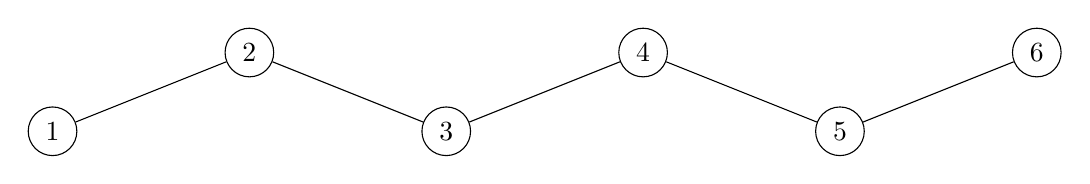
\begin{tikzpicture}
    
    \node[circle, draw=black] (v1) at  (0,-0.5) {1};
    \node[circle, draw=black] (v3) at  (2.5,0.5) {2};
    \node[circle, draw=black] (v7) at  (5,-0.5) {3};
    \node[circle, draw=black] (v4) at  (7.5,0.5) {4};
    \node[circle, draw=black] (v10) at  (10,-0.5) {5};
    \node[circle, draw=black] (v15) at  (12.5,0.5) {6};
    
    \draw[-] (v1)--(v3);
    \draw[-] (v3)--(v7);
    \draw[-] (v7)--(v4);
    \draw[-] (v4)--(v10);
    \draw[-] (v10)--(v15);


    \end{tikzpicture} 
    
        \begin{tikzpicture}
    
    \node[circle, draw=black] (v1) at  (0,-0.5) {1};
    \node[circle, draw=black] (v3) at  (2.5,0.5) {2};
    \node[circle, draw=black] (v7) at  (5,-0.5) {3};
    \node[circle, draw=black] (v4) at  (7.5,0.5) {4};
    \node[circle, draw=black] (v10) at  (10,-0.5) {5};
    \node[circle, draw=black] (v15) at  (12.5,0.5) {6};
    
    \draw[dashed] (v1)--(v3);
    \draw[dashed] (v3)--(v7);
    \draw[-] (v7)--(v4);
    \draw[dashed] (v4)--(v10);
    \draw[dashed] (v10)--(v15);

    \path [bend left] (v3) edge (v4);
    \path [bend left] (v3) edge (v15);

    \path [bend left] (v10) edge (v1);
    \path [bend left] (v10) edge (v7);


    
    \end{tikzpicture} 

    
    \caption{Troca de dois nós.}
    \label{fig:6}
\end{figure}


\section{Perturbações}
Buscar o melhor entre os vizinhos de uma solução pode prender um algoritmo em um ótimo local (uma solução que é melhor que todos os seus vizinhos), que não necessariamente é o ótimo global. Perturbações são, no geral, procedimentos que modificam uma drasticamente uma solução com a intenção de afastá-la de um ótimo local.

A perturbação utilizada por \cite{SILVA2012513} é chamada de \textit{double-bridge}, e pode ser pensada como a troca entre duas subsequências. Precisamente, é recomendado utilizar subsequências de interseção nula, geradas aleatoriamente, cujos tamanhos variam entre 2 e \(\frac{|V|}{10}\).

\section{Economia de operações}

Grande parte do tempo de execução do algoritmo se resume à avaliação dos movimentos através do cálculo de \(\Delta\). Evitar a realização de operações redundantes no processo é uma maneira de otimizá-lo, como ilustrado na Figura \ref{deltaCarroca}, que apresenta duas formas semelhantes de calcular o mesmo valor \texttt{A}.

\begin{figure}[!htbp]
    \centering
    \begin{lstlisting}
// Calculo com operacoes redundantes
for(int i = 0; i < n; i++)
{
    for(int j = 0; j < n; j++)
    {
       double A = (3 * i - 4) * j;
    }
}

// Calculo eficiente
for(int i = 0; i < n; i++)
{
    double B = (3 * i - 4);
    for(int j = 0; j < n; j++)
    {
       double A = B * j;
    }
}
    \end{lstlisting}
    \caption{Evitando operações redundantes.}
    \label{deltaCarroca}
\end{figure}

 Note que uma vez que o \textit{loop} interno se inicia, \texttt{i} não varia até que \texttt{j} assuma o valor \texttt{n}. Consequentemente, a operação \texttt{(3 * i - 4)}, será executada várias vezes, produzindo sempre o mesmo resultado. Isso pode ser evitado armazenando-se o valor dessa operação previamente, e utilizando-o no cálculo final de \texttt{A}.

\section{Parâmetros}
O número de tentativas de melhorar uma solução \(s\) no algoritmo de \cite{SILVA2012513} é determinado, principalmente, pelos parâmetros \(\text{I}_{\text{Max}}\) e \(\text{I}_\text{ILS}\). É recomendado utilizar \(\text{I}_{\text{Max}} = 50\) e \[\text{I}_\text{ILS} = \begin{cases}\frac{|V|}{2} \text{ se } |V| \geq 150 \\
            |V| \text{ senão}
            \end{cases}.\]
            
\section{Resultados}

A Tabela \ref{tabelaTempos} apresenta os valores médios de custo total \(f(s)\) e tempo de resolução de cada instância em 10 execuções do algoritmo, testado em um  Intel® Core™ i7-3770 3.40GHz.

\begin{table}

\begin{minipage}[b]{0.6\linewidth}
\scalebox{1}{
\begin{tabular}{lll}
\hline \\
Instância & tempo (s)   & \(f(s)\) \\
\hline \\
a280      & 96,623  & 2579    \\
ali535    & 1525    & 202384  \\
att48     & 0,3     & 10628   \\
att532    & 1778,96 & 27731   \\
bayg29    & 0,043   & 1610    \\
bays29    & 0,05    & 2020    \\
berlin52  & 0,374   & 7542    \\
bier127   & 10,209  & 118282  \\
brazil58  & 0,479   & 25395   \\
brg180    & 12,824  & 1950    \\
burma14   & 0,004   & 3323    \\
ch130     & 10,91   & 6110    \\
ch150     & 10,43   & 6528    \\
d198      & 33,639  & 15780   \\
d493      & 1132,48 & 35042   \\
dantzig42 & 0,161   & 699     \\
eil101    & 4,436   & 629     \\
eil51     & 0,369   & 426     \\
eil76     & 1,549   & 538     \\
fl417     & 365,503 & 11861   \\
fri26     & 0,033   & 937     \\
gil262    & 82,271  & 2378,7  \\
gr120     & 9,065   & 6942    \\
gr137     & 11,348  & 69853   \\
gr17      & 0,008   & 2085    \\
\hline 
\end{tabular}
}
\end{minipage}
\begin{minipage}[b]{0.7\linewidth}
\scalebox{1}{
\begin{tabular}{lll}
\hline \\
Instância & tempo (s)   & \(f(s)\) \\
\hline \\
gr202     & 37,105  & 40160,1 \\
gr21      & 0,014   & 2707    \\
gr229     & 61,498  & 134613  \\
gr24      & 0,028   & 1272    \\
gr431     & 721,745 & 171530  \\
gr48      & 0,314   & 5046    \\
gr96      & 3,475   & 55209   \\
hk48      & 0,336   & 11461   \\
kroA100   & 3,468   & 21282   \\
kroA150   & 11,751  & 26524   \\
kroA200   & 32,951  & 29368   \\
kroB100   & 3,748   & 22141   \\
kroB150   & 10,634  & 26130   \\
kroB200   & 35,53   & 29437,2 \\
kroC100   & 3,568   & 20749   \\
kroD100   & 4,114   & 21294   \\
kroE100   & 3,745   & 22068   \\
lin105    & 4,355   & 14379   \\
lin318    & 188,78  & 42045,7 \\
linhp318  & 187,536 & 42053,1 \\
pcb442    & 597,431 & 50876   \\
pr107     & 4,582   & 44303   \\
pr124     & 7,021   & 59030   \\
pr136     & 13,632  & 96772   \\
pr144     & 10,479  & 58537   \\
pr152     & 8,708   & 73682   \\
pr226     & 45,27   & 80369   \\
pr264     & 64,758  & 49135   \\
pr299     & 130,098 & 48194,8 \\
pr76      & 1,366   & 108159  \\
rat195    & 28,046  & 2326,1  \\
rat99     & 4,115   & 1211    \\
rd100     & 3,983   & 7910    \\
rd400     & 498,288 & 15296,1 \\
si175     & 17,333  & 21407   \\
si535     & 758,534 & 48466,8 \\
st70      & 1,03    & 675     \\
swiss42   & 0,155   & 1273    \\
ts225     & 28,869  & 126643  \\
tsp225    & 45,368  & 3916    \\
u159      & 10,828  & 42080   \\
ulysses16 & 0,008   & 6859    \\
ulysses22 & 0,019   & 7013   \\
\hline 
\end{tabular}
}
\end{minipage}
\caption{Tempos de execução e valores de custo total.}
\label{tabelaTempos}
\end{table} 


